\documentclass[11pt, a4paper]{article}

\usepackage[utf8]{inputenc}
\usepackage{fullpage}
\usepackage[parfill]{parskip} % Empty line instead of indentation
\usepackage{graphicx}
\graphicspath{ {images/} }
\usepackage{listings}
\usepackage{mathtools}
\usepackage{amssymb}
\usepackage{eurosym} %Euro symbol
%\usepackage[ngerman]{babel}
\usepackage{cancel} % Cancel fractions
\usepackage{units}
\usepackage{xcolor}
\usepackage{setspace}

\newcommand\braces[1]{\left(#1\right)}
\newcommand\brackets[1]{\left[#1\right]}
\renewcommand{\vec}[1]{\underline{#1}}
\newcommand{\mat}[1]{\underline{\underline{#1}}}
\newcommand{\abs}[1]{\left\lvert#1\right\rvert}
\newcommand{\norm}[1]{\left\lVert#1\right\rVert}
\newcommand\tr[1]{\mathrm{tr}\br{#1}}
\newcommand\average[1]{\left\langle#1\right\rangle}
\newcommand{\acos}[1]{\mathrm{acos}\braces{#1}}
\newcommand{\asin}[1]{\mathrm{asin}\braces{#1}}
\newcommand{\intend}[1][]{\ \mathrm{d}#1}
\newcommand{\derivative}[2][]{\ \frac{\mathrm{d}#1}{\mathrm{d}#2}} %\derivative[a]{b}
\newcommand\expectedValue[1]{\mathbb{E}\braces{#1}}
\newcommand\variance[1]{\mathbb{V}\braces{#1}}
\newcommand\setequal{\overset{!}{=}}
\newcommand{\gerquote}[1]{\glqq#1\grqq}
\definecolor{AI-BLUE}{rgb}{0,0.57,0.87}

\onehalfspacing
\setlength\parindent{0pt}
\allowdisplaybreaks

\title{TITLE}
\author{AUTHOR}
\date{\today}

\makeatletter
    \setlength\@fptop{0\p@}
\makeatother

\begin{document}
\thispagestyle{empty}

\begin{titlepage}
    \begin{center}
    \vphantom{0cm}
    \huge \textbf{Hardening artificial neural networks against specifically constructed adversarial input data} \\
    \vspace{4cm}
    %\LARGE \textbf{Report}\\
    \normalsize
    Written Master Thesis Report \\
    for the Masters Program of \textcolor{AI-BLUE}{[Applied Computer Science]}\\
    at the Ruhr-University Bochum\\
    in the Summer Term 2016\\
    \vspace{4cm}
    %\normalsize
    \textbf{Submitted by}\\
    B. Sc. Christian Andreas Mielers (108 011 204 956)\\
    \vspace{1cm}
    \today \\
    \vspace{1cm}
    \textbf{Supervisors} \\
    PD Dr. Rolf P. Würtz \\
    M. Sc. Andreas Nilkens
    \end{center}
\end{titlepage}

\newpage
\pagenumbering{arabic}
\setcounter{page}{2}

\tableofcontents

\newpage
\section{Introduction}
As the problems people try to solve with the aid of computers become more and more complex, their ability to write software that can keep up with those aspirations does not follow suit. Solving more complex problems with software does not only incur the cost of finding viable solutions and formalizing them in computer code, but also the cost of integrating all the necessary components, organizing their interactions, ensuring they use common resources in a well-defined manner, and testing all of the above. These tasks grow essentially super-linearly in difficulty, and can thus quickly become harder than the problem that the system was initially meant to solve.

One way out of this dilemma that people turn to increasingly often is the usage of machine learning techniques. The goal of machine learning is to free people from the burden of finding and programming a solution. In order to do so, a \emph{model} is defined which embodies the structure of a possible solution on a highly abstract level. However, such a model as potentially a myriad of \emph{parameters}, and no knowledge of reasonable values for those parameters can be assumed. What gives machine learning its name and makes it feasible despite the many unknown parameters is the learning method. This is a method to find a working configuration of parameters based on \emph{training data}. In \emph{supervised learning}, the algorithm that performs the learning is provided numerous pairs of an exemplary input and the corresponding desired output that the model should deliver. From these pairs, it extracts, or \emph{learns}, the relationship between input and output data, and codifies it in the model's parameters. In this manner, the need for a handcrafted solution is eliminated. The downside to this approach is that learning algorithms usually require a copious amount of training data to find good parameters. However, this drawback is increasingly often offset by the reduced software complexity, since machine learning models usually have a well-defined theoretical foundation with ready-made software available.
% TODO write something about verification with test data?

% TODO substantiate claim that ANNs are among the top machine learning models
Among some of the most momentous machine learning models are \emph{artificial neural networks (ANNs)}. They are inspired by discoveries from the field of neural biology and incorporate them into models that, on a very abstract level, resemble brain structures on the detail level of individual neurons. The workings of these  neuron are greatly simplified, but in this way they can be easily connected in large bulks, empowering the resulting network to solve difficult tasks with impressive precision. ANNs are mainly used to two types of tasks: \emph{classification} and \emph{regression}. While the latter is concerned with learning a function $f: X \rightarrow Y$ that maps input data to the desired output values, it is the former that will be of interest within the scope of this thesis. Classification instead aims to assign each input to one category out of a predefined set of categories. The data used to train the network is structured accordingly: it consists of the input data and a \emph{label} that denotes its class.
% TODO note that learner for neural networks is "gradient descent"?

% TODO illustrate image classification
One area where neural networks are particularly successful is \emph{image classification}, the task of classifying an object by from a digital photo of it. A big part of the success here can be attributed to a special variant of ANNs, called \emph{Convolutional Neural Networks (CNNs)}. These networks focus on local features in the input by applying \emph{filters} in a convolution operation, thereby curtailing redundancies in the free parameters. Combined with the focus on local features, this efficient use of free parameters allows for much larger and thus more powerful networks.

% TODO illustrate training and test steps with an image
When training a neural network for an image classification task, one desires a CNN to not only classify the images used for training correctly, but to infer and learn the fundamental characteristics of each class. Only then will the network be able to \emph{generalize} its classification capabilities to the previously unseen images it will encounter in productive use. To gauge a network's ability to generalize, another data set, called the \emph{test set} is usually withheld while training the model. The experimenter can then evaluate the performance on this set outside of training, thus obtaining an estimator for field performance of the model.

In the past, ANNs in general and CNNs in particular have shown convincing results not only on training data but also test data. However, recent discoveries have indicated that the generalization capability of most neural networks is not as strong as one might guess from test set performance. While networks certainly can classify unseen input with high reliability, it is possible to find minute transformations of correctly classified test data, on which the network will predict another class with high confidence. The changes that need to be applied for this to work are miniscule and undetectable to the human eye. The resulting images are called \emph{adversarial examples (AEs)}.

In the initial publication a rather complex method for creating those images was presented. A major impediment of this method was the excessive computational power and time required to produce AEs. Fortunately, a follow-up paper greatly improved the feasibility of this process by introducing a gradient-based procedure for generating AEs. In that manner a considerable amount of AEs can be generated in a reasonable time frame, enough to allow for reasonable quantitative analysis of the AE's properties. Therefore, this thesis will look at various statistics of larger groups of AEs, including their spectra and the ways these spectra differ from those of unadulterated images. Regarding the spectra, we will also look at the distribution of values with regards to the frequency and orientation.

Furthermore, the process of generating adversarial examples can be inspected on a considerably larger scale. Plots for the network confidence on images in the process of being turned into AEs will provide insights on the process with regards to iteration count, and serve as the foundation for attempts to predict whether an image can be successfully made adversarial. Data on the success rate of converting images to adversarial examples will be presented, both per original and adversarial class as well as overall figures.

The aforementioned results will be obtained with multiple data sets and various network layouts and parameter configurations. The latter will also allow for inspection of the impact of parameter choice on various statistics.

% History
% What is a neural network
% Strengths
% Industry applications
% The problem with adversarial examples
% What this thesis is about
% Future prospects

\newpage
\section{Artificial Neural Networks}
In the area of machine learning, artificial neural networks are some of the most widely studied models. They stem from insights into the workings of real, biological brains in the field of neural biology. Here, the individual neuron is used as the fundamental unit of computation. A schematic version of the biological variant is shown in figure \ref{fig:biological-neuron-schematic}.

\begin{figure}[htp]
	\centering
	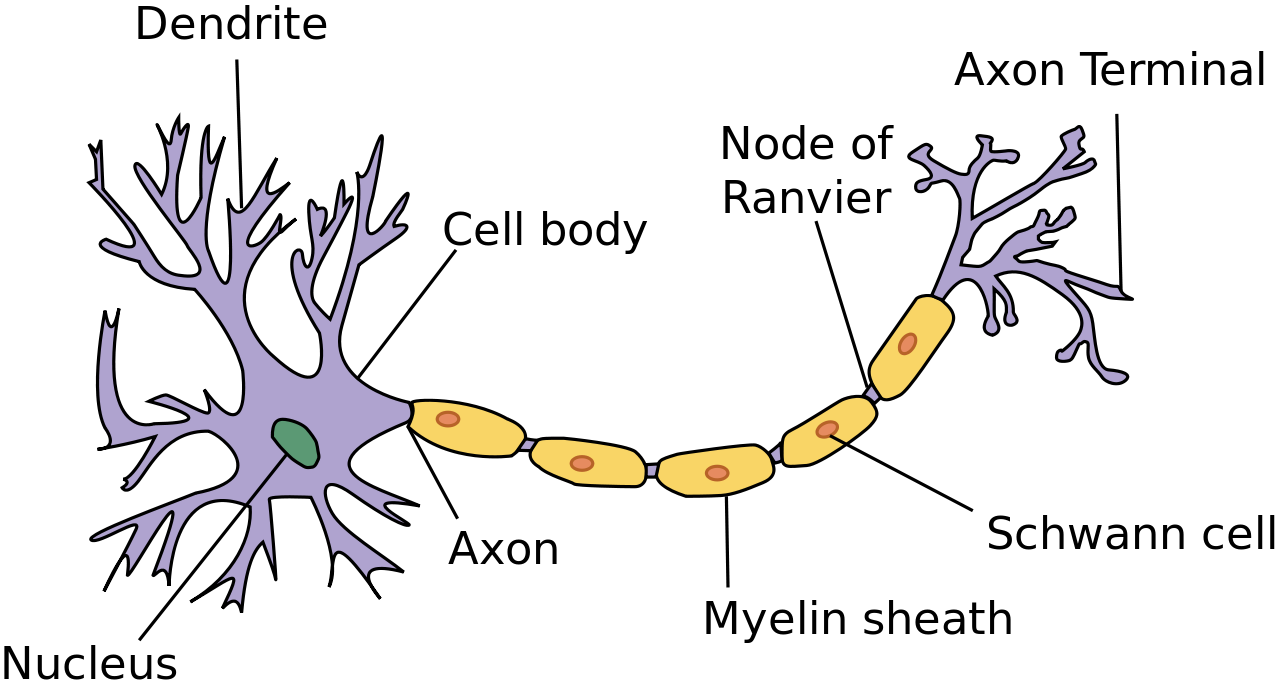
\includegraphics[width=0.5\textwidth]{images/biological_neuron.png}
	\caption{Schematic of a biological neuron, taken from \cite{biological-neuron-schematic}}
	\label{fig:biological-neuron-schematic}
\end{figure}

% TODO be a bit more precise here with the chemistry
A neuron receives incoming electrical pulses, called \emph{action potentials}, from the axons of other neurons via its dendrites. A connection between an axon and a dendrite is called a \emph{synapse}. These synapses can vary in strength, so the intensity of the received pulse is modulated by the synaptic connectivity. Multiple action potentials may arrive in the soma, the cell body of a neuron, in quick succession, causing the membrane potential of the soma to increase. If enough action potentials arrive within a short time via strong synapses, this may cause the cell in question to initiate an action potential which traverses along its axon. This can be considered to be a decision of the sell to pass the message on to other cells.

An artificial neuron as used in an ANN mimics this process, but in a greatly simplified form. All action potential rates are represented by real numbers\footnote{Floating point numbers in a computer system}. A visual representation is provided in figure \ref{fig:artificial-neuron-schematic}.


\begin{figure}[htp]
	\centering
	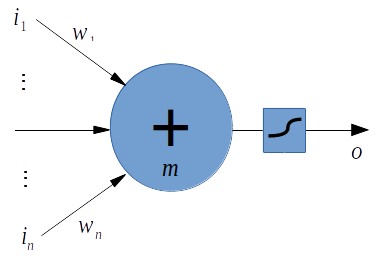
\includegraphics[width=0.45\textwidth]{images/artificial_neuron.png}
	\caption{Schematic of an artificial neuron}
	\label{fig:artificial-neuron-schematic}
\end{figure}

The first thing to note is that the input to the neuron is now formalized as a vector $\vec{i}$ with components $i_1 \dots i_n$, where $n$ represents the number of inputs that influence this neuron. Each input value $i_j$ is multiplied with a \emph{weight}, denoted by $w_j$. This weight can be thought of as an abstraction of the synaptic strength between two neurons. Then, all of these input-weight pairs are summed up to realize the counterpart to the membrane potential, labeled $m$. To form the neuron's output $o$, one last step is neccessary. In biological neurons, the rate of outgoing spikes of a neuron is not linear in the incomming spikes. Thus, a nonlinear \emph{activation function} is applied to the membrane potential $m$, symbolized by the sigmoidally shaped line in the rectangular box in figure \ref{fig:artificial-neuron-schematic}. If that activation function is called $\sigma$, the mathematical operation performed by a single neuron can be summarized according to equations \eqref{neuron-math-membrane-potential} and \eqref{neuron-math-activation-function}.

\begin{align}
	m &= \sum_{i=1}^n w_n \cdot i_n = \vec{w}^T \vec{i} \label{neuron-math-membrane-potential}\\
	o &= \sigma \braces{m} \label{neuron-math-activation-function}
\end{align}



% TODO will it only become especially important in chapter 3, or also in other places?
Take note of the fact that the very first step performed on the input is essentially an inner product. This will become important later on, especially in chapter \ref{sec:adversarial-examples}. Several activation functions are possible. A plot of 3 common choices is given in figure \ref{fig:activation-functions}.

\begin{figure}[htp]
	\centering
	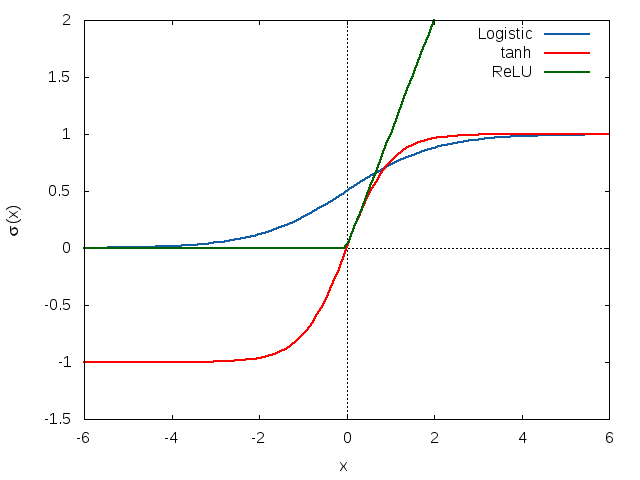
\includegraphics[width=0.6\textwidth]{images/activation_functions.png}
	\caption{Logistic sigmoidal, hyperbolic tangent and ReLU activation functions}
	\label{fig:activation-functions}
\end{figure}

Out of these, the easiest to justify is the logistic sigmoid. If the output is to represent the neuron's firing rate, it must not become negative, and it must saturate because of the refractory period required by biological cells. Under these conditions, the logistic function is a simple continuous choice. The hyperbolic tangent is a linearly transformed version of this. While its negative range may be harder to interpret biologically, the option to output negative values may relieve the trainable parameters of a network of some demand for computational power, thus facilitating training. Despite being non-continuous and having no upper bound, the ReLU is the most popular activation function according to \cite{deep-learning-2015}. The networks utilized in this thesis mostly make use of the $\tanh$ and ReLU activation functions.

Since a single neuron as described above consists only of an inner product and a onedimensional non-linearity, its computational power is limited. Artificial neural networks rely on thousands of neurons to perform their tasks. This gives rise to the question of how to connect all those neurons. Conceptually, one could link them up in such a way that a neuron that receives input from another neuron while at the same time delivering input to that same neuron (either directly or via proxy neurons), forming a cycle. This is sometimes done in practice and is called a \emph{Recurrent Neural Network (RNN)}, but is out of scope for this thesis. Instead, neurons will be organized in \emph{layers}, as shown in figure %TODO

Here, each layer contains numerous neurons, all of which are not connected to one another.

% The activation function's nonlinearity is what gives a network its power.

% Biologically inspired
% Very popular
% Successful
% Neuron is a radial simplification % Disregard of time
% Some math
% Layered
% Activation functions
% Error function
% Gradient descent
% Deep learning
% Recurrent vs. feed-forward

\subsection{Convolutional Neural Networks}
A special kind of ANN that has proven to be particularly effective on image data is the \emph{Convolutional Neural Network (CNN)}.

% Training with gradient descent

\section{Adversarial Examples}
\label{sec:adversarial-examples}
% Generalization across different models and data sets
% They tried to use AEs to train the network to be more resistant, didn't work
% Theoretical ramifications for human vision
% How does the explanation given in "Harnessing AEs" relate to CNNs?
% Linear explanation for AE's existence



% Googlenet

\bibliographystyle{alpha}
\bibliography{ref,image_ref}

\end{document}

% List of figures
% List of tables
% List of acronyms

















